\documentclass[a4paper]{article}

\usepackage[UTF8]{ctex}
\usepackage[a4paper,margin=1in]{geometry}
\usepackage{graphicx}
\usepackage{float}
\usepackage{listings}
\usepackage{longtable}
\usepackage{booktabs}
\usepackage{hyperref}
\usepackage{fancyhdr}
\usepackage{lastpage}
\usepackage{color}
\usepackage{xcolor}
\usepackage{indentfirst}        % 首段缩进
\setlength{\parindent}{2em}     % 缩进2字符
\usepackage{zhnumber}           % 中文编号
\usepackage[dvipsnames]{xcolor}
\usepackage{amsmath}
\usepackage{multimedia}  % 添加多媒体支持
\usepackage{qrcode}      % 添加二维码支持(可选)
\usepackage[most]{tcolorbox}  % 添加彩色框支持
%\newcommand{\college}{中山大学计算机学院}
\newcommand{\projname}{计算机图形学|作业三}
\newcommand{\reporttitle}{Phong shading与VBO绘制三维物体及其性能分析}
\newcommand{\stuno}{23336179}
\newcommand{\authorname}{马福泉}
\newcommand{\major}{计算机科学与技术}
\newcommand{\adviser}{陶钧}
\newcommand{\startdate}{2025年12月10日}
\newcommand{\labenddate}{2025年12月20日}
\newcommand{\labroom}{B402}

\pagestyle{fancy} % 使用 fancyhdr 风格
\fancyhf{}      % 清空默认的页眉页脚

% 设置页眉
\fancyhead[L]{\kaishu \projname}      % 左侧页眉显示项目名称
\fancyhead[C]{\kaishu \reporttitle}    % 中间页眉显示报告标题
\fancyhead[R]{\kaishu \authorname} % 右侧页眉显示作者姓名

% 设置页脚
\fancyfoot[C]{第 \thepage 页，共 \pageref{LastPage} 页} % 中间页脚显示页码

% 去除页眉页脚与正文之间的分隔线
\renewcommand{\headrulewidth}{0.4pt}
\renewcommand{\footrulewidth}{0pt}

% 设置文档背景颜色
\definecolor{mybgcolor}{RGB}{0, 0, 0} % 定义背景颜色
\definecolor{NavyBlue}{RGB}{0,0,128} % 添加颜色定义
% \pagecolor{mybgcolor} % 设置背景颜色

\lstset{
    basicstyle=\ttfamily\small,
    commentstyle=\color{gray},
    keywordstyle=\color{blue},
    stringstyle=\color{red},
    breaklines=true,
    frame=single,
    numbers=left,
    numberstyle=\tiny\color{gray},
    tabsize=4,
    showstringspaces=false,
    captionpos=b,
    language=C++
}

\begin{document}

% 封面
\begin{titlepage}
    \centering
    

    
\includegraphics[width=10cm]{img/SYSULogo.png}

    \vspace{1em}
    %{\Large \college \par}
    \vspace{1em}
    {\Large \kaishu \projname \par}
    \vspace{3em}

    

    
    {\fontsize{40pt}{42pt}\kaishu \selectfont \boldmath \reporttitle\par}
    \vspace*{\fill}

    \begin{center}
    {\Large
    \makebox[5em][s]{学号}:\underline{\makebox[15em][c]{\kaishu \stuno}}\\[1em]
    \makebox[5em][s]{姓名}:\underline{\makebox[15em][c]{\kaishu \authorname}}\\[1em]
    \makebox[5em][s]{专业}:\underline{\makebox[15em][c]{\kaishu \major}}\\[1em]
    \makebox[5em][s]{课程教师}:\underline{\makebox[15em][c]{\kaishu \adviser}}\\[1em]
    \makebox[5em][s]{起始日期}:\underline{\makebox[15em][c]{\kaishu \startdate}}\\[1em]
    \makebox[5em][s]{结束日期}:\underline{\makebox[15em][c]{\kaishu \labenddate}}\\[1em]
    \makebox[5em][s]{实验地点}:\underline{\makebox[15em][c]{\kaishu \labroom}}
    }
    \end{center}

    \vspace*{\fill}
\end{titlepage}

% 目录
\tableofcontents
\newpage

% 实验报告正文开始

\section{实验概述}

本实验主要实现了基于 Phong 着色模型的三维物体渲染，并采用 VBO（顶点缓冲对象）进行高效绘制。具体内容如下：

\begin{itemize}
    \item \textbf{Phong shading 实现}：通过 fragment shader 实现 Phong shading。首先在 vertex shader 中输出法向量，GLSL 自动对法向量进行插值并传递给 fragment shader，最终在 fragment shader 中根据 Phong 模型计算环境光、漫反射和镜面反射三类分量，实现真实感光照。
    \item \textbf{VBO 绘制三维物体}：使用 VBO 存储顶点数据和连接关系（如索引数组），可通过细分物体（如小球）生成大量三角面片，实现复杂三维模型的高效渲染。
    \item \textbf{相关对比与讨论}：
    \begin{enumerate}
        \item 对比 Phong shading 与 OpenGL 自带的 smooth shading（如 Gouraud 着色）的区别，分析两者在光照计算精度和视觉效果上的差异。
        \item 对比使用 VBO 绘制与传统 glVertex 方式的区别，讨论 VBO 在性能和数据管理上的优势。
        \item （选做）实现并讨论 VBO 是否使用索引数组（index array）对效率的影响。
        \item （选做）对比、讨论 HW3（本实验）与 HW2 的渲染结果和效率差别。
    \end{enumerate}
\end{itemize}

\section{实现过程}
\subsection{实验环境}
\subsubsection{实验环境及其存在的问题分析}
\textbf{实验环境现状}
库构成：GLFW（窗口与上下文）、ImGui（UI）、GLM（数学库）。
定义宏：CMake 中显式定义了 \texttt{IMGUI\_IMPL\_OPENGL\_LOADER\_GL3W}。
核心配置：CMake 链接了 \texttt{OpenGL::GL} 和 \texttt{opengl32.lib}。

\textbf{存在的核心问题}
\begin{itemize}
    \item \textbf{符号缺失}：Windows 自带的 \texttt{opengl32.lib} 只导出 OpenGL 1.1 版本的函数。像 \texttt{glGenBuffers}、\texttt{glVertexAttribPointer} 这种现代 OpenGL 函数属于“扩展”，它们在动态库中只有地址，没有静态导出符号。
    \item \textbf{加载器失效}：由于项目中实际上没有 \texttt{gl3w.c} 源码，虽然在 CMake 声明了要用它，但编译器找不到其实现。
    \item \textbf{头文件冲突}：如果不手动声明，编译器就会报“未定义标识符”的错误。
\end{itemize}
\subsubsection{自定义函数指针等解决}
这种方法本质上是\textbf{模拟加载器（Loader）}的工作原理：手动从显卡驱动程序（DLL）中查询函数地址并赋值给全局变量。
\textbf{解决步骤}：
\begin{enumerate}
    \item \textbf{声明函数指针类型}：根据 OpenGL 官方规范，定义这些函数的类型。可直接在 \texttt{main.cpp} 顶部声明。
    \item \textbf{定义全局函数变量}：定义与 OpenGL 函数同名的函数指针变量。
    \item \textbf{使用 \texttt{glfwGetProcAddress} 运行时加载}：在 \texttt{glfwMakeContextCurrent(window)} 之后，通过 GLFW 的 API 获取函数的真实物理地址。
\end{enumerate}
\vspace{1em}
\subsubsection{解决方案代码（部分）}
\begin{lstlisting}[language=C++,caption={main.cpp 关键代码}]
#include <GLFW/glfw3.h>
#include <iostream>
// --- 1. 手动定义缺失的宏和函数指针类型(部分)---
#define GL_ARRAY_BUFFER                   0x8892
#define GL_STATIC_DRAW                    0x88E4
#define GL_FRAGMENT_SHADER                0x8B30

typedef void (APIENTRYP PFNGLGENBUFFERSPROC) (GLsizei n, GLuint *buffers);
typedef void (APIENTRYP PFNGLBINDBUFFERPROC) (GLenum target, GLuint buffer);
typedef void (APIENTRYP PFNGLBUFFERDATAPROC) (GLenum target, GLsizeiptr size, const void *data, GLenum usage);
// --- 2. 定义全局函数指针对象 ---
PFNGLGENBUFFERSPROC               glGenBuffers = nullptr;
PFNGLBINDBUFFERPROC               glBindBuffer = nullptr;
PFNGLBUFFERDATAPROC               glBufferData = nullptr;
// --- 3. 编写加载函数 ---
void loadOpenGLFunctions() {
    glGenBuffers = (PFNGLGENBUFFERSPROC)glfwGetProcAddress("glGenBuffers");
    glBindBuffer = (PFNGLBINDBUFFERPROC)glfwGetProcAddress("glBindBuffer");
    glBufferData = (PFNGLBUFFERDATAPROC)glfwGetProcAddress("glBufferData");
    glGenVertexArrays = (PFNGLGENVERTEXARRAYSPROC)glfwGetProcAddress("glGenVertexArrays");
    glBindVertexArray = (PFNGLBINDVERTEXARRAYPROC)glfwGetProcAddress("glBindVertexArray");
    glVertexAttribPointer = (PFNGLVERTEXATTRIBPOINTERPROC)glfwGetProcAddress("glVertexAttribPointer");
    glEnableVertexAttribArray = (PFNGLENABLEVERTEXATTRIBARRAYPROC)glfwGetProcAddress("glEnableVertexAttribArray");
}
int main() {
    if (!glfwInit()) return -1;
    GLFWwindow* window = glfwCreateWindow(800, 600, "Manual Pointer Loading", NULL, NULL);
    glfwMakeContextCurrent(window);
    // 关键：必须在创建上下文后加载地址
    loadOpenGLFunctions();
    // 之后你就可以正常使用 glGenBuffers(1, &VBO) 等函数了，不再报错
    return 0;
}
\end{lstlisting}

\subsection{实验思路}
本实验基于 OpenGL 核心模式（Core Profile），旨在通过可编程管线（Programmable Pipeline）实现高真实感的 Phong 光照模型，并利用 VBO（顶点缓冲对象）技术解决高精度模型的实时渲染效率问题。以下从光照计算、几何构建、性能优化三个维度阐述实验思路与代码实现逻辑。
\subsubsection{Phong 光照模型的着色器实现思路}
Phong 模型的核心思想是将光照分解为环境光（Ambient）、漫反射（Diffuse）和镜面反射（Specular）三个分量。为了实现“逐像素”的平滑光照（即 Phong Shading），核心计算逻辑放置在片元着色器（Fragment Shader）中，而非顶点着色器。
\textbf{（1）数据准备与法线变换（Vertex Shader 逻辑）}
在进行光照计算前，需确保法向量（Normal）在世界空间中的正确性。数学原理上，物体发生非均匀缩放时，法向量不能直接乘以模型矩阵 $M$，否则会失去与切平面的垂直性。因此需计算法线矩阵 $G$：
$$
G = (M^{-1})^T
$$
代码实现时，在 Vertex Shader 中，输入顶点坐标 aPos 乘以 $MVP$ 矩阵输出 gl\_Position。关键在于用 \texttt{mat3(transpose(inverse(uModel)))} 计算法线矩阵，将属性 aNormal 变换到世界坐标系赋值给输出变量 vNormal，随后由光栅化器自动插值传递给 Fragment Shader。

\textbf{（2）逐像素光照计算（Fragment Shader 逻辑）}
在 Fragment Shader 中，需计算三个核心光照分量。所有参与计算的向量（光线方向 $\vec{L}$、法线 $\vec{N}$、视线 $\vec{V}$）均需归一化处理。

A. \textbf{环境光（Ambient）}
公式：$I_{amb} = k_a \cdot I_{light}$
实现：定义常量系数（如 0.1），乘以光源颜色 uLightColor，模拟全局散射光，确保背光面不会死黑。

B. \textbf{漫反射（Diffuse）}
公式：$I_{diff} = k_d \cdot I_{light} \cdot \max(\vec{N} \cdot \vec{L}, 0)$
实现：获取插值后的法线 vNormal 并归一化为 $\vec{N}$，用光源位置 uLightPos 减去片元位置 vWorldPos 得到 $\vec{L}$，用 \texttt{dot(N, L)} 计算点积并截断负值，确保只有面向光源的面被照亮。

C. \textbf{镜面反射（Specular）}
公式：$I_{spec} = k_s \cdot I_{light} \cdot (\max(\vec{V} \cdot \vec{R}, 0))^{\alpha}$
实现：计算视线向量 $\vec{V}$（相机位置 uViewPos 减去片元位置），反射向量 $\vec{R}$ 用 \texttt{reflect(-L, N)} 得到。高光强度为 $\vec{V}$ 与 $\vec{R}$ 的点积幂运算，反光度由 Uniform 变量 uShininess 控制。

D. \textbf{最终合成}
将 ambient、diffuse、specular 叠加，乘以物体材质基色 uObjectColor，输出为最终片元颜色 FragColor。

\subsubsection{基于 VBO 的球体网格生成与存储}
为验证 VBO 在处理大量几何图元时的优势，采用数学参数化方法生成高细节度球体模型。

\textbf{（1）几何细分与三角面片生成}
数学原理：利用球坐标系方程，遍历经度角 $\theta \in [0, 2\pi]$ 和纬度角 $\phi \in [0, \pi]$ 生成顶点：
\[
\begin{cases}
x = r \sin\phi \cos\theta \\
y = r \cos\phi \\
z = r \sin\phi \sin\theta
\end{cases}
\]
代码实现时，C++ 的 makeSphere 函数用双层 for 循环，外层控制纬度（Stacks），内层控制经度（Slices）。顶点生成时，$(i, j)$ 计算 $(\phi, \theta)$，代入公式求 $(x, y, z)$，压入 std::vector。单位球体法向量即为归一化坐标，直接复用。拓扑连接时，将相邻四点 $(i, j), (i+1, j), (i, j+1), (i+1, j+1)$ 组合成两个三角形，索引存入索引数组。

\textbf{（2）VBO 与 EBO 的显存管理}

不同于立即模式每帧由 CPU 发送数据，本实验采用“一次上传，多次绘制”策略。缓冲创建用 glGenVertexArrays 和 glGenBuffers，数据上传用 glBindBuffer 和 glBufferData，将 std::vector 数据传递给 GPU，指定 GL\_STATIC\_DRAW 优化显存布局。属性指针配置用 glVertexAttribPointer，前3个 float 为 Position，后3个为 Normal，实现数据与渲染逻辑解耦。

\subsubsection{渲染模式的对比分析思路}

\textbf{（1）Phong Shading vs. Gouraud Shading}

对比思路：验证光照计算阶段对画质的影响。实现时通过 Uniform 变量 uShadingMode 控制 Shader 分支。uShadingMode==1（Gouraud）时，光照计算在 Vertex Shader，Fragment Shader 仅插值颜色；uShadingMode==0（Phong）时，Vertex Shader 仅传递法线，Fragment Shader 逐像素计算。预期差异：Gouraud 模式高光呈现棱角，Phong 模式高光圆润。

\textbf{（2）VBO Indexed vs. Immediate Mode}

对比思路：验证“数据驻留显存”与“CPU 逐帧发送”的效率差异。渲染循环中通过 drawMode 变量切换：VBO 路径用 glDrawElements，CPU 只发一次指令，GPU 利用 VRAM 数据高速绘制；Immediate 路径关闭 Shader，回退 OpenGL 1.1 固定管线，每帧用 glBegin/glEnd 包裹数万次 glVertex3f，模拟高频 CPU-GPU 通信，直观展示传统 API 性能瓶颈

\subsubsection{核心渲染耗时的精确统计机制}

本实验放弃了仅依靠 FPS（每秒帧数）来衡量性能的方法，因为 FPS 往往受到垂直同步（V-Sync）的钳制（通常锁定在 60FPS）以及 ImGui 界面绘制开销的干扰，无法真实反映图形管线的核心性能。
为了精确量化不同渲染模式的效率差异，我们采用了以下统计策略：
\begin{itemize}
    \item \textbf{高精度计时}：使用 \texttt{glfwGetTime()} 获取微秒级的时间戳。
    \item \textbf{计时范围}：仅记录核心绘制指令（Draw Calls）和着色器 Uniform 设置的耗时。严格排除 ImGui 界面构建、\texttt{glfwPollEvents} 以及 \texttt{glfwSwapBuffers} 的时间。这样能真实反映 CPU 提交渲染命令的开销以及 GPU 的处理延迟（在同步模式下）。
    \item \textbf{平滑处理}：为了方便观察，采用“累积平均法”，每累计 60 帧计算一次平均单帧耗时（Avg Core Render Time），避免数值跳动过快影响读数。
\end{itemize}

\subsection{代码实现}
本节展示实验的核心代码实现，涵盖了光照模型的着色器编写、几何数据的生成与管理，以及不同渲染模式的运行时逻辑。

\subsubsection{Phong 光照模型 (Fragment Shader)}
该片段着色器实现了完整的 Phong 光照计算。它接收光栅化阶段插值后的法向量和位置，逐像素计算光照强度。
\begin{lstlisting}[language=C++,caption={Phong Fragment Shader}]
#version 330 core
out vec4 FragColor;

// 顶点着色器传递的插值变量
in vec3 vNormal;
in vec3 vWorldPos;

// Uniform 全局变量
uniform vec3 uLightPos;
uniform vec3 uViewPos;
uniform vec3 uLightColor;
uniform vec3 uObjectColor;
uniform float uShininess;

void main() {
    // 1. 环境光 (Ambient)
    float ambientStrength = 0.1;
    vec3 ambient = ambientStrength * uLightColor;

    // 2. 漫反射 (Diffuse)
    vec3 norm = normalize(vNormal);
    vec3 lightDir = normalize(uLightPos - vWorldPos);
    float diff = max(dot(norm, lightDir), 0.0);
    vec3 diffuse = diff * uLightColor;

    // 3. 镜面高光 (Specular)
    float specularStrength = 0.5;
    vec3 viewDir = normalize(uViewPos - vWorldPos);
    vec3 reflectDir = reflect(-lightDir, norm);
    float spec = pow(max(dot(viewDir, reflectDir), 0.0), uShininess);
    vec3 specular = specularStrength * spec * uLightColor;

    // 最终颜色合成
    vec3 result = (ambient + diffuse + specular) * uObjectColor;
    FragColor = vec4(result, 1.0);
}
\end{lstlisting}
\textbf{代码说明}：\\
vNormal 和 vWorldPos 是从顶点着色器传递并经过 GPU 自动线性插值后的数据，确保了光照在曲面上的平滑过渡。所有方向向量均需归一化。环境光防止背光面全黑，漫反射基于 Lambert 余弦定律，镜面光用反射向量与视线夹角的幂模拟高光。

\subsubsection{球体细分与 VBO 数据生成 (C++)}
该函数通过数学参数化生成高细节的球体网格数据，包含顶点位置、法线以及用于绘制三角形的索引。
\begin{lstlisting}[language=C++,caption={球体网格生成}]
Mesh makeSphere(unsigned stacks, unsigned slices, float radius) {
    Mesh m;
    // 1. 顶点生成
    for (unsigned i = 0; i <= stacks; ++i) {
        float phi = (float(i) / stacks) * PI; // 纬度角 [0, PI]
        for (unsigned j = 0; j <= slices; ++j) {
            float theta = (float(j) / slices) * 2.0f * PI; // 经度角 [0, 2PI]
            float x = radius * sinf(phi) * cosf(theta);
            float y = radius * cosf(phi);
            float z = radius * sinf(phi) * sinf(theta);
            m.vertices.push_back(x); m.vertices.push_back(y); m.vertices.push_back(z);
            m.vertices.push_back(x/radius); m.vertices.push_back(y/radius); m.vertices.push_back(z/radius);
        }
    }
    // 2. 索引生成
    for (unsigned i = 0; i < stacks; ++i) {
        for (unsigned j = 0; j < slices; ++j) {
            unsigned k1 = i * (slices + 1) + j;
            unsigned k2 = k1 + slices + 1;
            m.indices.push_back(k1); m.indices.push_back(k2); m.indices.push_back(k1 + 1);
            m.indices.push_back(k2); m.indices.push_back(k2 + 1); m.indices.push_back(k1 + 1);
        }
    }
    return m;
}
\end{lstlisting}

\textbf{代码说明}：\\
利用双层循环遍历经纬度，将球坐标 $(\phi, \theta)$ 转换为笛卡尔坐标 $(x, y, z)$，法线直接用归一化坐标。索引缓冲区（EBO）存储连接关系，避免重复顶点。

\subsubsection{VBO 数据上传与绑定 (C++)}
该函数负责 OpenGL 缓冲对象的创建、绑定以及将 CPU 端的几何数据传输至 GPU 显存。

\begin{lstlisting}[language=C++,caption={VBO/EBO 上传与属性绑定}]
GLMesh uploadMesh(const Mesh& m) {
    GLMesh gm;
    glGenVertexArrays(1, &gm.vao);
    glGenBuffers(1, &gm.vbo);
    glGenBuffers(1, &gm.ebo);

    glBindVertexArray(gm.vao);

    glBindBuffer(GL_ARRAY_BUFFER , gm.vbo);
    glBufferData(GL_ARRAY_BUFFER , m.vertices.size() * sizeof(float), m.vertices.data(), GL_STATIC_DRAW);

    glBindBuffer(GL_ELEMENT_ARRAY_BUFFER , gm.ebo);
    glBufferData(GL_ELEMENT_ARRAY_BUFFER , m.indices.size() * sizeof(unsigned int), m.indices.data(), GL_STATIC_DRAW);

    glVertexAttribPointer(0, 3, GL_FLOAT , GL_FALSE , 6 * sizeof(float), (void*)0);
    glEnableVertexAttribArray(0);

    glVertexAttribPointer(1, 3, GL_FLOAT , GL_FALSE , 6 * sizeof(float), (void*)(3 * sizeof(float)));
    glEnableVertexAttribArray(1);

    glBindVertexArray(0);
    return gm;
}
\end{lstlisting}

\textbf{代码说明}：\\
用 glGenBuffers 和 glBufferData 将 std::vector 数据拷贝到 GPU 显存，属性采用交错存储：[x, y, z, nx, ny, nz]，位置和法线分别对应不同 attribute location。

\subsubsection{绘制循环中的模式对比 (VBO vs Immediate)}
展示如何在运行时动态切换“现代 VBO 绘制”与“传统立即模式绘制”，以验证性能差异。

\begin{lstlisting}[language=C++,caption={渲染模式切换}]
if (drawMode == 0) { // VBO (Indexed)
    glUseProgram(prog);
    glUniformMatrix4fv(..., modelMatrix);
    glBindVertexArray(mesh.vao);
    glDrawElements(GL_TRIANGLES , mesh.indexCount , GL_UNSIGNED_INT , 0);
}
else if (drawMode == 2) { // 立即模式 (Legacy OpenGL)
    glUseProgram(0);
    glBegin(GL_TRIANGLES);
    for (size_t i = 0; i < mesh.vertices.size(); i += 6) {
        glNormal3f(mesh.vertices[i+3], mesh.vertices[i+4], mesh.vertices[i+5]);
        glVertex3f(mesh.vertices[i],    mesh.vertices[i+1], mesh.vertices[i+2]);
    }
    glEnd();
}
\end{lstlisting}

\textbf{代码说明}：\\
VBO 模式下，CPU 只需一次 draw call，GPU 并行处理显存数据。立即模式下，CPU 每帧遍历所有顶点并逐个发送，通信开销大，效率低，便于直观对比现代与传统渲染方式。

\subsubsection{核心渲染时间统计逻辑}
为了获取纯净的渲染耗时，我们在渲染循环中植入了计时探针。
\begin{lstlisting}[language=C++,caption={核心渲染耗时统计}]
// 变量定义
double renderTimeAccum = 0.0;
int renderFrameCount = 0;
float displayRenderTime = 0.0f;

// 渲染循环内部
double tStart = glfwGetTime(); // [计时开始]

if (drawMode != 2) {
    // VBO 模式绘制逻辑...
    glUseProgram(prog);
    // ... 设置 Uniforms ...
    glBindVertexArray(mesh.vao);
    glDrawElements(GL_TRIANGLES, mesh.indexCount, GL_UNSIGNED_INT, 0);
} else {
    // 立即模式绘制逻辑...
    glUseProgram(0);
    glBegin(GL_TRIANGLES);
    // ... glVertex3f 循环 ...
    glEnd();
}
double tEnd = glfwGetTime();   // [计时结束]
// 累积计算
renderTimeAccum += (tEnd - tStart) * 1000.0; // 转换为毫秒
renderFrameCount++;
if (renderFrameCount >= 60) {
    displayRenderTime = (float)(renderTimeAccum / renderFrameCount);
    renderTimeAccum = 0.0;
    renderFrameCount = 0;
}
\end{lstlisting}
\textbf{代码说明}：\\
该代码段通过调用 \texttt{glfwGetTime()} 记录渲染开始和结束的时间，计算出每帧的渲染耗时（单位为毫秒）。通过累积 60 帧的时间并求平均，得到较为稳定的核心渲染时间指标，便于性能对比分析。

\subsection{结果与分析}

本实验基于 OpenGL Core Profile 架构，通过编写 GLSL 着色器实现了高真实感的 Phong 光照模型，并利用 VBO 技术高效绘制了高精度的球体模型。实验最后对比了不同渲染策略及历史作业（HW2）的性能差异。

\subsubsection{通过 Fragment Shader 实现 Phong Shading}

\textbf{实验结果}

在控制面板中选择 "Phong (Pixel)" 模式，渲染结果如下图所示。可以看到球体表面呈现出细腻的光照过渡。特别是高光（Specular）区域，光斑边缘圆润平滑，且随着光源移动，光斑在曲面上的形变自然，无明显的几何棱角感。

\begin{figure}[H]
    \centering
    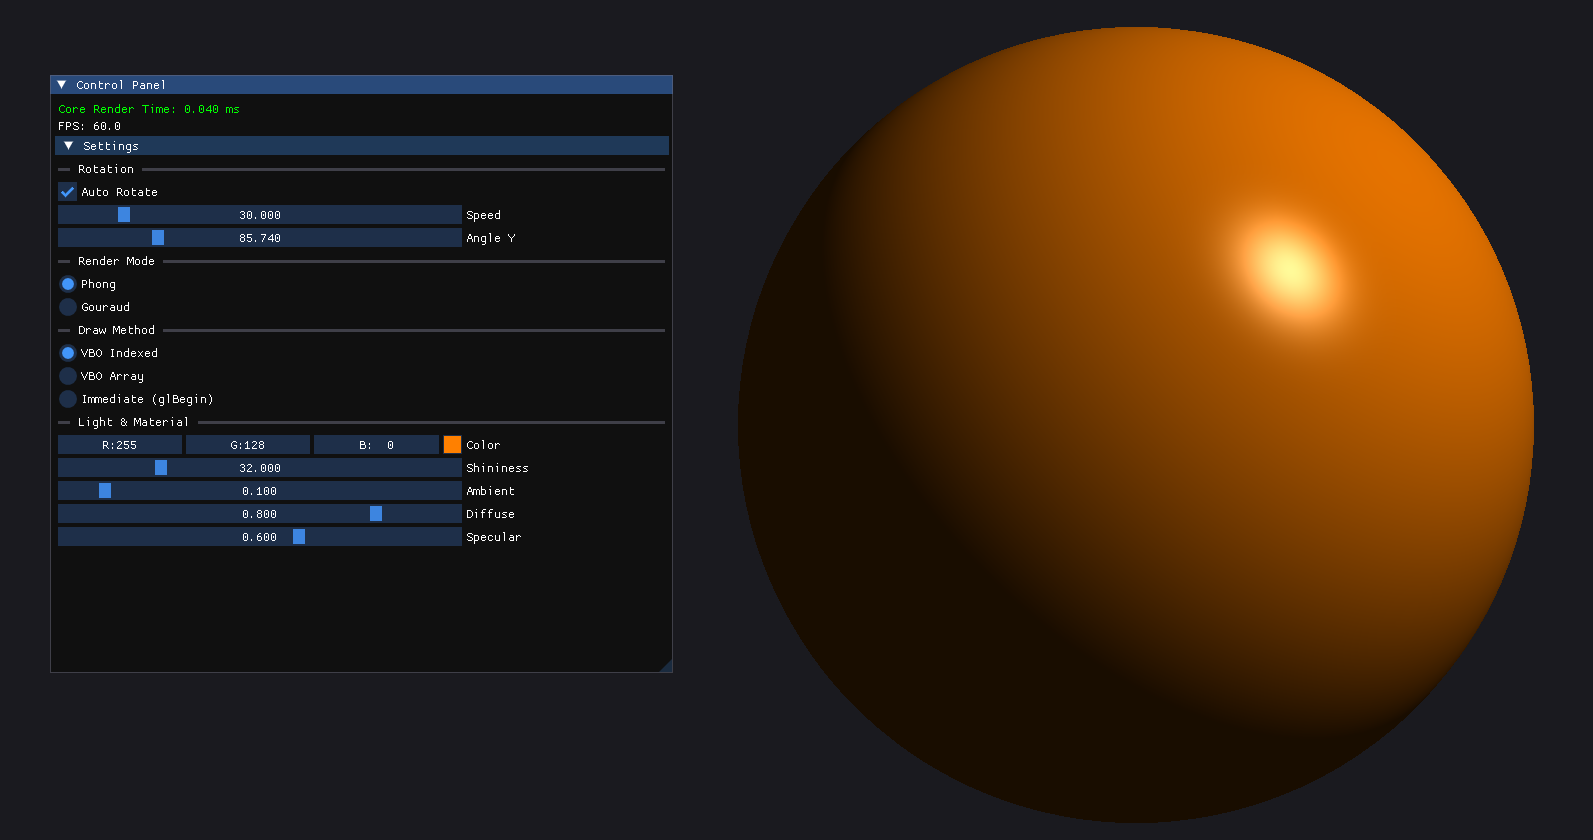
\includegraphics[width=0.45\textwidth]{img/phong_render_full.png}
    \caption{Phong 模式下的球体渲染结果}
\end{figure}

\textbf{结果分析}

Phong Shading 的高真实感得益于其在片元（像素）级别进行的计算流程，而非顶点级别。

\begin{itemize}
    \item \textbf{法向量输出 (Vertex Shader)}：在顶点着色器中，使用法线矩阵 \texttt{mat3(transpose(inverse(uModel)))} 变换法线，确保了非均匀缩放下的几何正确性。
    \item \textbf{自动插值 (Rasterization)}：GPU 光栅化阶段自动对三角形顶点的法线进行线性插值，使得 Fragment Shader 接收到的 \texttt{vNormal} 是平滑连续的。
    \item \textbf{三类反射计算 (Fragment Shader)}：在片元着色器中实现了完整的 Phong 公式。由于计算发生在每个像素上，即使三角形面片较大，高光也能精确地落在三角形内部，呈现出完美的圆形。
\end{itemize}

\subsubsection{使用 VBO 存储顶点与连接关系}

\textbf{物体细分与网格生成}

实验通过参数化方程 \texttt{makeSphere} 生成球体。为了直观验证细分逻辑对模型精度的影响，我们对比了高细节与低细节两种参数下的渲染结果。
高细节模式 (64x64)：如下图所示，当细分参数设为 stacks=64, slices=64 时，网格极其致密（约 8000+ 三角形），球体边缘光滑，逼近理想曲面。

\begin{figure}[H]
    \centering
    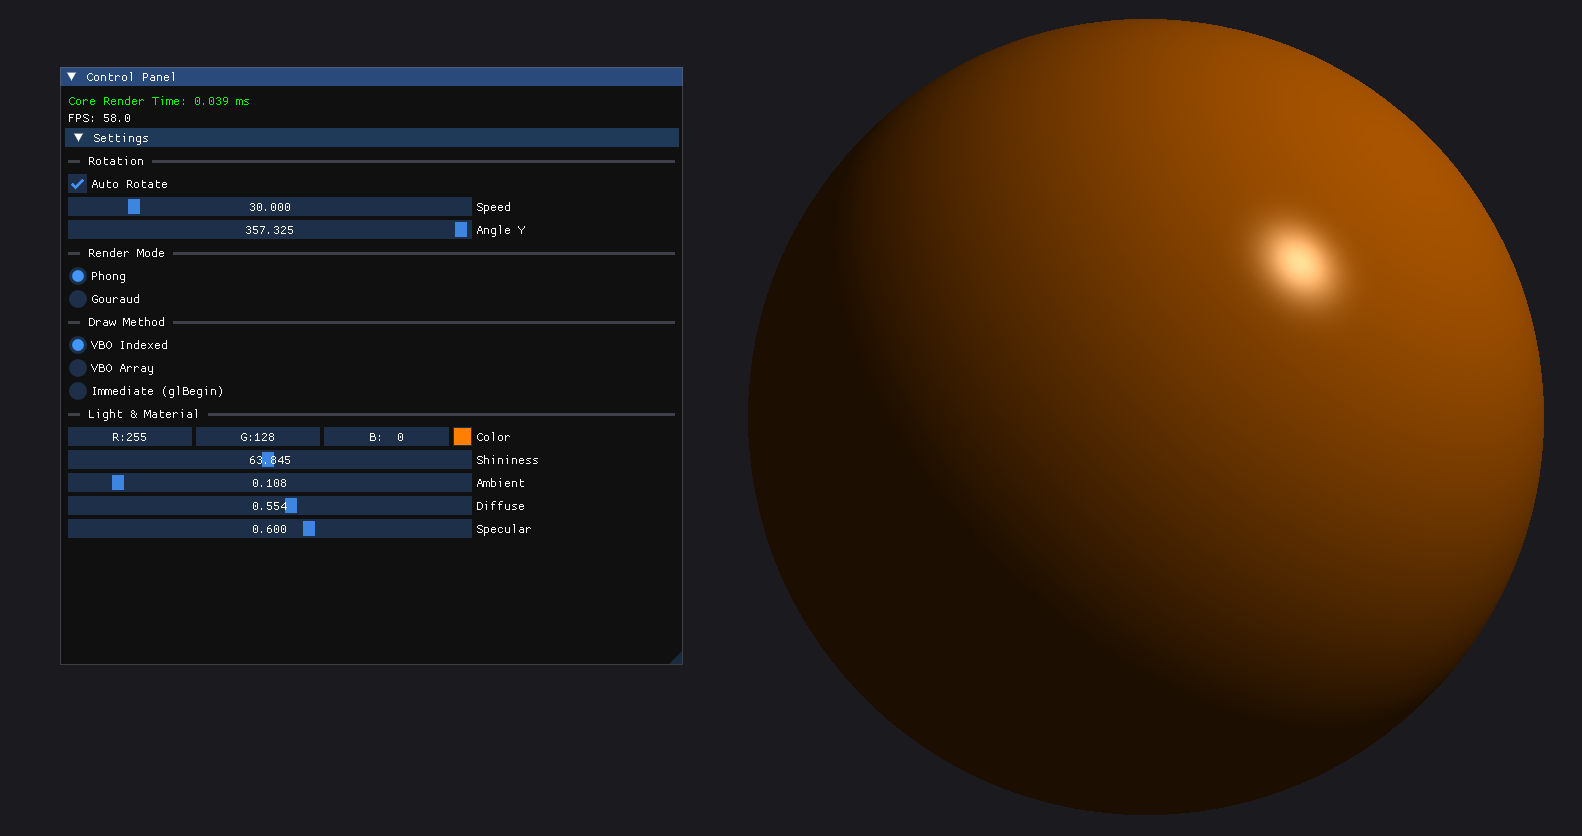
\includegraphics[width=0.45\textwidth]{img/sphere_smooth_detail.png}
    \caption{高细节球体（64x64）}
\end{figure}
中细节模式 (验证细分逻辑)：我们将细分参数降低至 stacks=8, slices=8 并重新编译运行。如下图所示，球体表面出现了明显的“棱角”和多边形轮廓。这直观地证明了我们的 VBO 正确存储了由 \texttt{makeSphere} 函数动态生成的离散三角面片数据，而非加载了预制的模型。

\begin{figure}[H]
    \centering
    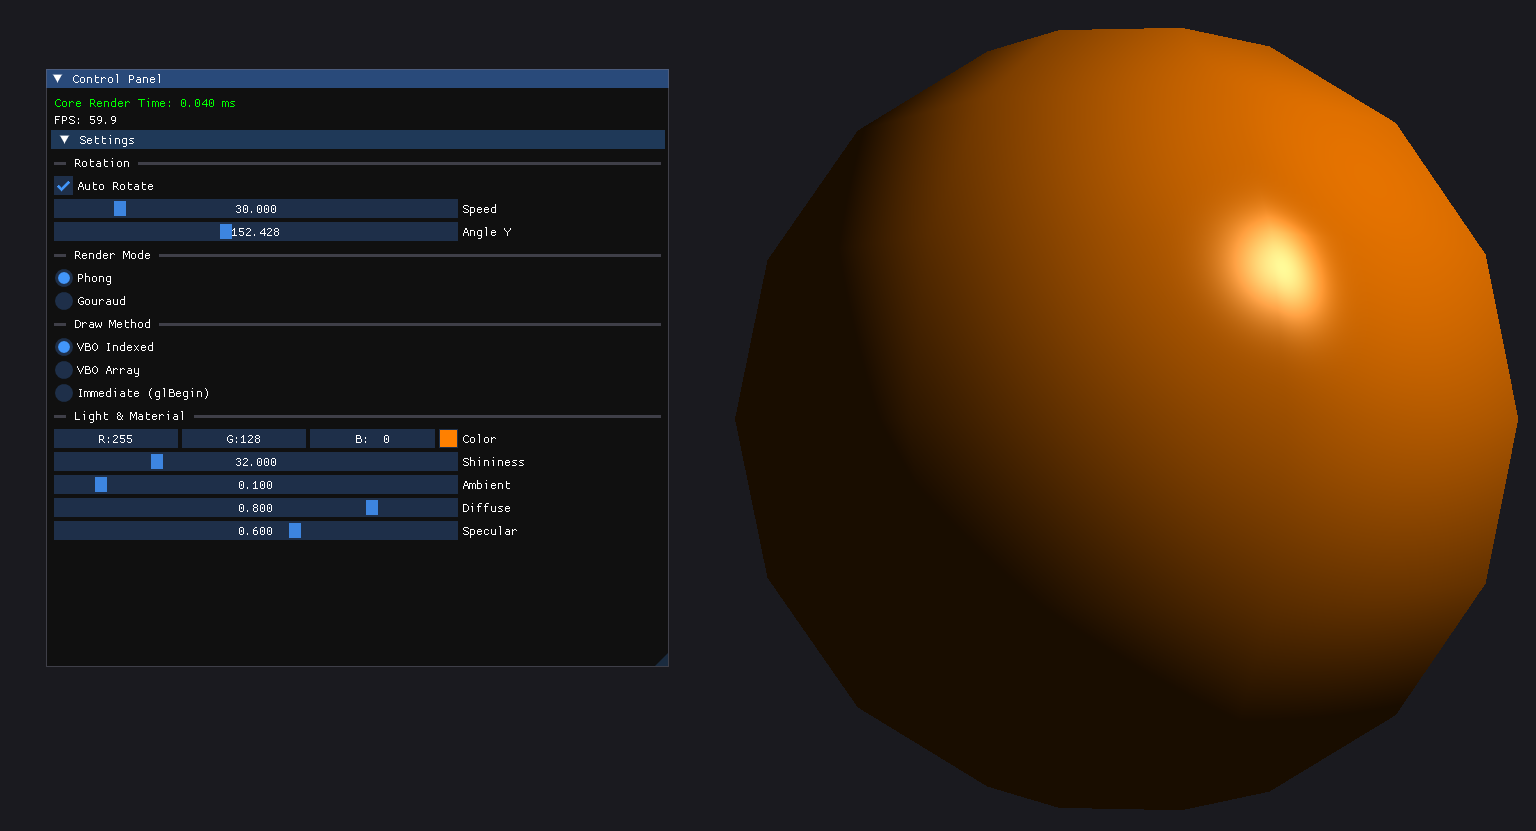
\includegraphics[width=0.45\textwidth]{img/sphere_low_poly.png}
    \caption{低细节球体（8x8），可见明显三角面片}
\end{figure}
低细节模式 (验证细分逻辑)：我们将细分参数降低至 stacks=4, slices=4 并重新编译运行。如下图所示，球体表面出现了更加明显的“棱角”和多边形轮廓。这进一步验证了我们的 VBO 正确存储了由 \texttt{makeSphere} 函数动态生成的离散三角面片数据。
\begin{figure}[H]
    \centering
    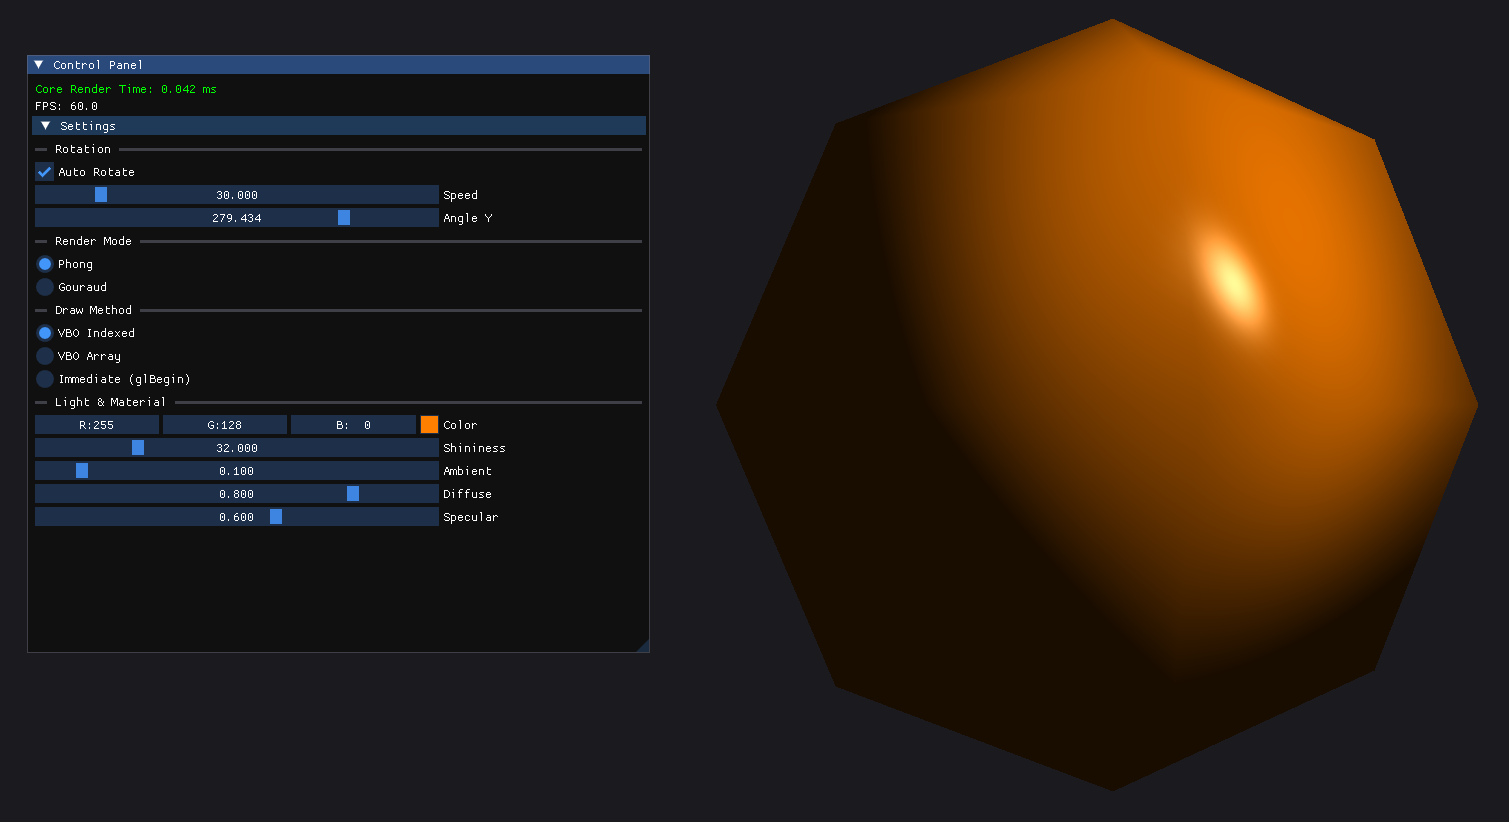
\includegraphics[width=0.45\textwidth]{img/sphere_very_low_poly.png}
    \caption{极低细节球体（4x4），可见更加明显三角面片}
\end{figure}

\subsubsection{对比实验}

\textbf{对比 Phong Shading 与 OpenGL 自带 Smoothing Shading 的区别}

我们通过 \texttt{uShadingMode} 切换 Shader 逻辑，模拟了传统的 Gouraud Shading（顶点光照）。

\begin{figure}[H]
    \centering
    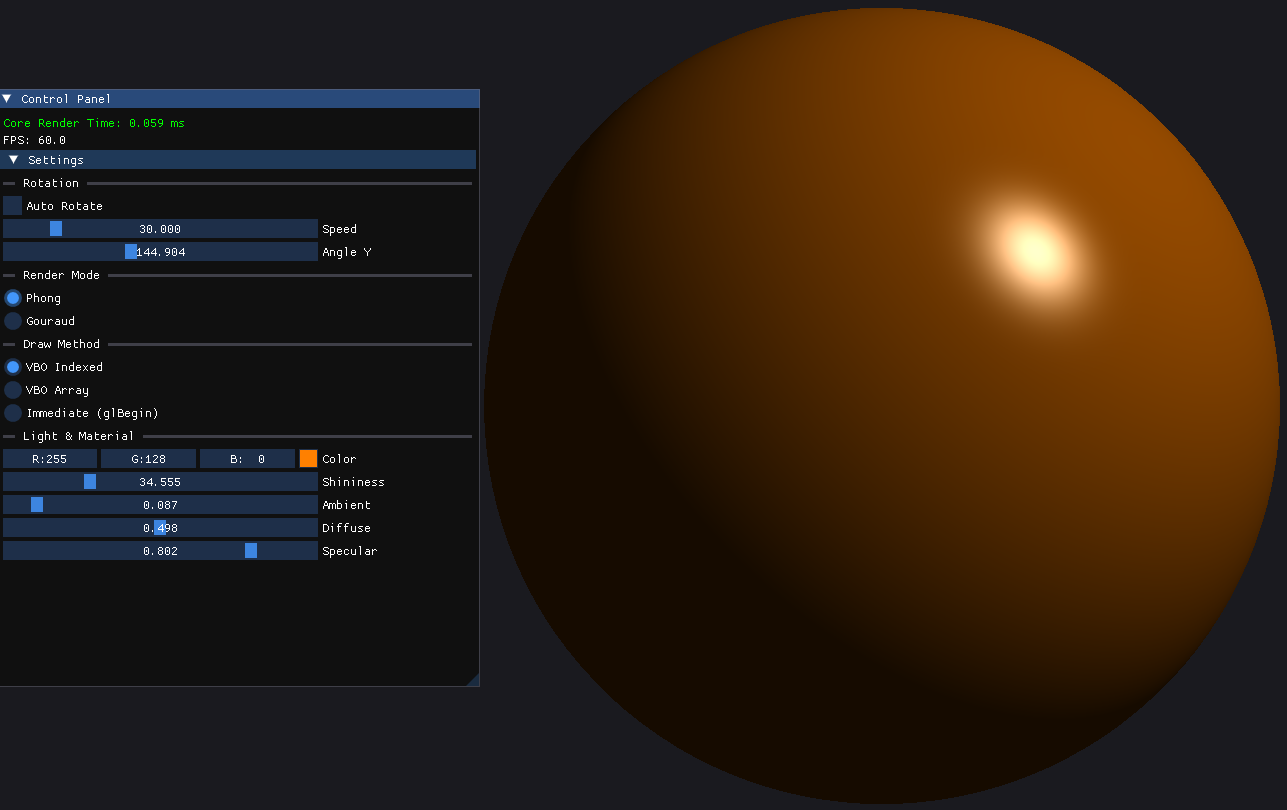
\includegraphics[width=0.45\textwidth]{img/phong_specular_closeup.png}
    \hspace{1em}
    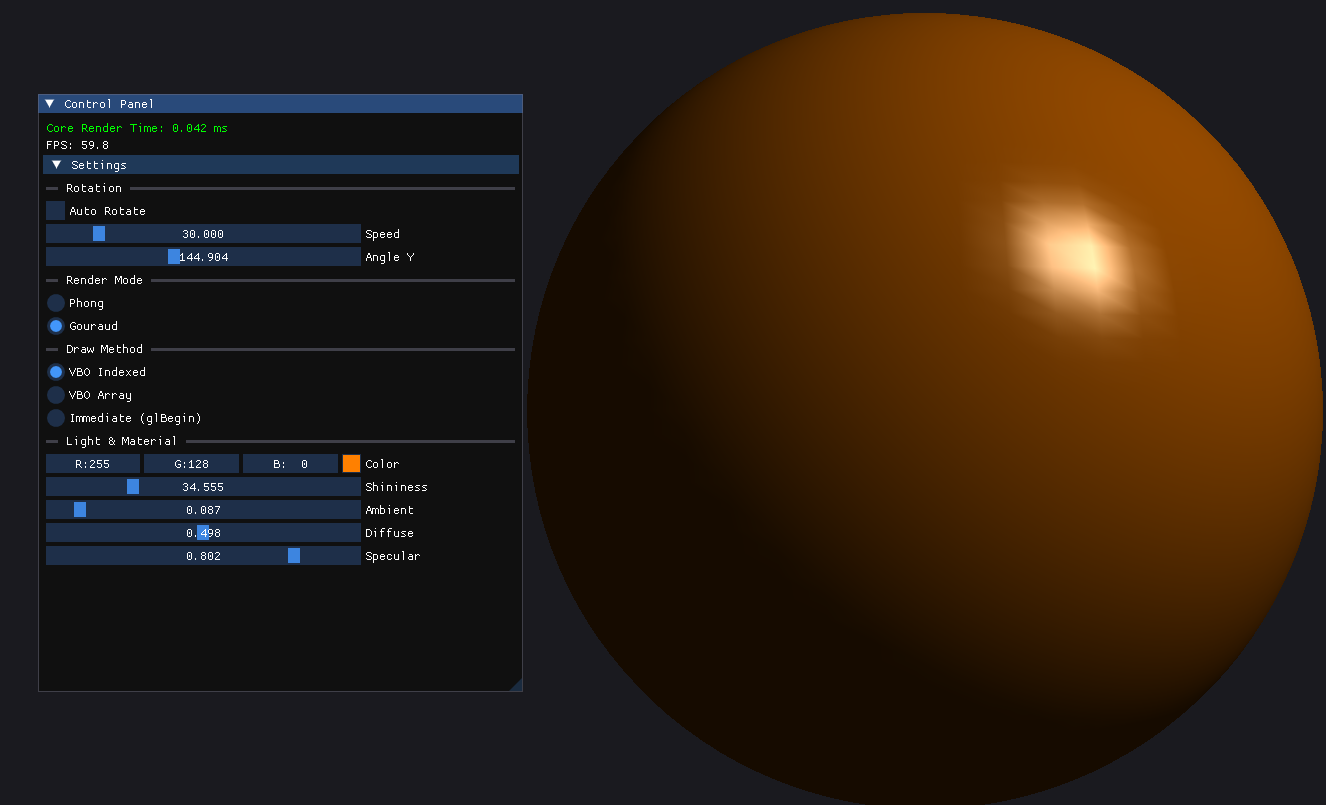
\includegraphics[width=0.45\textwidth]{img/gouraud_specular_closeup.png}
    \caption{左：Phong 高光 \quad 右：Gouraud 高光}
\end{figure}

分析：Phong 模式下的高光是完美的圆形；而 Gouraud 模式下的高光呈现出明显的菱形或星形棱角（Mach Band 效应）。这是因为 Gouraud 只在顶点计算光照颜色并进行线性插值，当高光区域小于网格面片时，插值算法无法重建高光中心的亮度峰值。

\textbf{使用 VBO 进行绘制及通过 glVertex 进行绘制的区别}

本实验通过控制面板切换绘制路径，并利用高精度计时器统计了 "Core Render Time"（核心渲染耗时），以此对比 "VBO Mode" 与 "Immediate Mode" 的性能差异。

\textbf{VBO 模式 (GPU 驱动)}：
如下图所示，在开启 VBO 时，核心渲染耗时维持在极低水平（约 0.05 ms）。这是因为 CPU 每一帧仅需发送一条 \texttt{glDrawElements} 指令，几乎没有 CPU 负载，数据传输瓶颈被消除，渲染效率极高。

\begin{figure}[H]
    \centering
    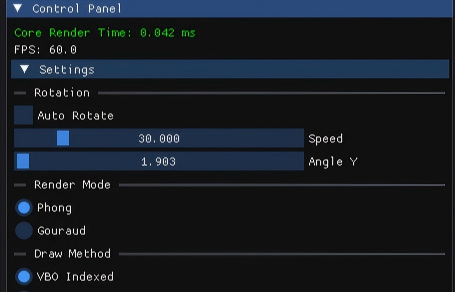
\includegraphics[width=0.45\textwidth]{img/render_time_vbo.png}
    \caption{VBO 模式下的核心渲染耗时（约 0.05ms）}
\end{figure}

\textbf{Immediate Mode (CPU 驱动)}：
如下图所示，切换到立即模式后，核心渲染耗时显著上升至 1 ms 左右（增长了约 30 倍）。

\begin{figure}[H]
    \centering
    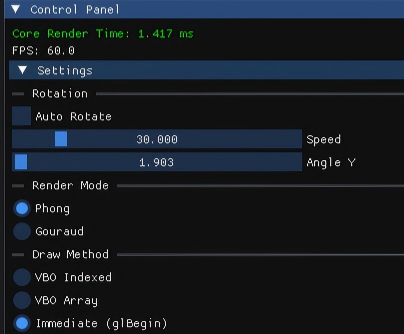
\includegraphics[width=0.45\textwidth]{img/render_time_immediate.png}
    \caption{Immediate Mode 下的核心渲染耗时（上升至 ms 级别）}
\end{figure}

\textbf{深度分析（为何 FPS 没有下降？）}：
值得注意的是，在实验机器上，立即模式下的 FPS 可能依然维持在 60 FPS 左右。这主要是受垂直同步（V-Sync）的限制，且当前的球体模型面数（约 8000 面）尚未达到 CPU 的处理极限。CPU 依然有能力在 16.6ms（60Hz 帧周期）的截止时间内完成数万次 \texttt{glVertex} 调用并提交给 GPU。

然而，Core Render Time 的剧增揭示了其低效的本质：立即模式每一帧都需要 CPU 执行海量的函数调用并进行频繁的内存-显存数据搬运。这种模式极大地浪费了 CPU 资源。一旦场景复杂度继续增加（例如渲染数百个球体），立即模式的耗时将迅速突破 16.6ms 导致 FPS 骤降，而 VBO 模式由于数据驻留显存，仍能保持极高的运行效率。

\subsubsection{(选做) VBO 中是否使用 Index Array 的效率量化讨论}

\begin{figure}[H]
    \centering
    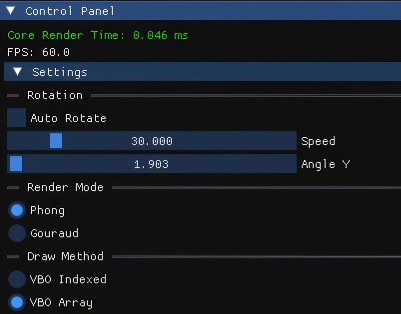
\includegraphics[width=0.6\textwidth]{img/render_time_vbo_array.png}
    \caption{VBO 模式下的核心渲染耗时（极低）}
\end{figure}

\textbf{分析要点}：

从上图可以看出，在 VBO 模式下，Core Render Time 极低（通常在 0.05ms 左右）。这表明 CPU 提交 \texttt{glDrawElements} 指令几乎是瞬间完成的，且是非阻塞的。

虽然在简单的球体模型上，Indexed 绘制与 Array 绘制在时间数值上难以看出显著区别（都极快），但从理论和硬件架构角度分析，Indexed 模式具有决定性优势：
\begin{itemize}
    \item \textbf{显存带宽 (Memory Bandwidth)}：Indexed 模式通过 EBO 复用顶点。对于共享顶点的网格（如球体），顶点数量通常比索引数量少得多。使用索引可以减少约 50\% 的顶点数据传输和显存占用。
    \item \textbf{Post-Transform Cache 优化}：GPU 拥有变换后顶点缓存。当索引重复出现时，GPU 可以直接读取缓存中已经执行过 Vertex Shader 的结果，而无需重新计算。这是 Array 模式无法做到的。
\end{itemize}

\subsubsection{(选做)HW3 (硬件渲染) 与 HW2 (软件渲染) 的跨实验对比}

为了直观展示硬件加速的威力，我们将 HW2（纯 CPU 软件光栅化）、HW3 立即模式（CPU 发送 + GPU 绘制）与 HW3 VBO 模式（GPU 全托管）进行了横向对比：

\begin{table}[H]
    \centering
    \begin{tabular}{|c|c|c|c|}
    \hline
    \textbf{实验项目} & \textbf{渲染模式} & \textbf{典型单帧耗时} & \textbf{主要瓶颈} \\
    \hline
    HW2 & 软件光栅化 & 20 $\sim$ 200 ms & CPU 算力（逐像素计算） \\
    \hline
    HW3 & 立即模式 (Immediate) & 1$\sim$2ms & CPU-GPU 总线带宽（逐顶点发送） \\
    \hline
    HW3 & VBO 模式 & 0.02$\sim$0.05 ms & 无（GPU 并行计算） \\
    \hline
    \end{tabular}
    \caption{不同渲染架构的性能对比}
\end{table}

\textbf{深度结论}：

\begin{enumerate}
    \item \textbf{HW2 vs HW3 (CPU 串行 vs GPU 并行)}：
    HW2 的耗时主要源于 CPU 需要对屏幕上的每一个像素进行插值和着色计算。对于 $800 \times 600$ 的窗口，这是 48 万次计算，CPU 的串行架构难以负载。而 HW3 利用 GPU 的数千个流处理器并行工作，实现了质的飞跃。
    
    \item \textbf{Immediate vs VBO (带宽瓶颈)}：
    即使使用了 GPU（如 HW3 立即模式），如果数据传输方式不当，效率依然低下。立即模式下，CPU 每帧都要通过总线发送数万个顶点数据，导致 GPU 大部分时间在“等待数据”。而 VBO 模式将数据驻留在显存中，彻底消除了 CPU-GPU 之间的通信带宽瓶颈，释放了硬件的全部潜能。
\end{enumerate}

\section{实验总结}
\subsection{实验完成情况说明}
本次实验按照要求全部完成了基于现代 OpenGL 核心模式（Core Profile）的各项功能，具体完成情况如下：
\begin{itemize}
    \item \textbf{光照模型实现}：成功编写了 GLSL 顶点与片元着色器，实现了完整的 Phong 光照模型，包括环境光（Ambient）、漫反射（Diffuse）与镜面反射（Specular）三个分量的精确计算。
    \item \textbf{几何生成与管理}：实现了球体网格的参数化生成算法，支持动态调整细分精度（Stacks/Slices），并通过 VBO 与 EBO 将顶点属性与索引数据一次性上传至显存。
    \item \textbf{多维度对比分析}：
    \begin{enumerate}
        \item 视觉层面：对比了 Phong Shading 与 Gouraud Shading 的渲染差异，验证了逐像素着色在处理高光细节上的优越性。
        \item 性能层面：对比了 VBO（Indexed/Array）与传统立即模式（Immediate Mode）的效率。
    \end{enumerate}
    \item \textbf{性能量化（选做）}：利用 \texttt{glfwGetTime} 剥离了 UI 渲染与缓冲区交换的干扰，实现了“核心渲染耗时（Core Render Time）”的统计功能，量化了 GPU 并行架构与 CPU 串行提交的性能鸿沟。
\end{itemize}

\subsection{主要收获}

通过本次实验，我在理论知识与工程实践两方面均取得了显著收获：
\begin{itemize}
    \item \textbf{管线思维的转变}：深刻理解了从“固定管线”到“可编程管线”的思维跨越。掌握了如何通过 Shader 控制图形管线的各个阶段，实现了对渲染流程的底层掌控。
    \item \textbf{显存管理与优化意识}：掌握了 VBO/EBO 的生命周期管理，理解了减少 CPU-GPU 通信（降低 Draw Call Overhead）是现代图形程序优化的核心。数据驻留显存的机制是实现复杂场景实时渲染的基石。
    \item \textbf{数学原理的具象化}：从数学层面掌握了法线矩阵变换（逆转置矩阵）的必要性，以及 Phong 反射向量计算的几何原理，将抽象的线性代数公式转化为了直观的视觉效果。
\end{itemize}

\subsection{困难与解决}

在实验过程中，我遇到了若干技术挑战，并通过查阅文档与逻辑推导逐一解决：
\begin{itemize}
    \item \textbf{环境配置与加载器失效}：在 CMake 配置中，由于缺少 \texttt{gl3w} 源码导致现代 OpenGL 函数符号无法链接。
    \textbf{解决}：我编写了一个 Mini-Loader，利用 \texttt{glfwGetProcAddress} 在运行时手动加载了 \texttt{glGenBuffers}、\texttt{glBufferData} 等核心函数指针，成功避开了对第三方加载库的依赖，加深了对 OpenGL 扩展加载机制的理解。
    \item \textbf{立即模式下的变换逻辑异常}：在实现立即模式对比时，发现球体绕摄像机公转而非自转。
    \textbf{解决}：通过重新分析矩阵乘法顺序，意识到在 OpenGL 栈操作中必须遵循 $V \times M \times v$ 的变换逻辑。修正为先载入视图矩阵（View）再乘以模型矩阵（Model）后，旋转效果恢复正常。
    \item \textbf{性能分析的量化误差}：初期仅观察 FPS，受垂直同步（V-Sync）限制，VBO 与立即模式均锁定在 60FPS，无法体现性能差异。
    \textbf{解决}：修改统计逻辑，剥离了 ImGui 绘制与 \texttt{SwapBuffers} 的阻塞时间，单独统计核心渲染循环的耗时。最终成功观测到 VBO（<0.05ms）与立即模式（>1ms）之间数十倍的效率差距，使实验结论更具说服力。
\end{itemize}

\end{document}